\chapter{Math: Complex Analysis} 

Here we review some basics of complex analysis that often appear in physics
calculation. Some useful resources for this include
Ref.~\cite{brown_complex_2003,weber_essentials_2012}.

\section{Preliminaries}\label{sec:complexPrelim}

We are interested in functions $f:\C\to\C$. Derivatives are defined similarly as
with real, $1D$ functions. The limit
\begin{equation}\label{eq:cderiv}
  \dv{f}{z}\equiv\lim_{w\to z}\frac{f(w)-f(z)}{w-z}
\end{equation}
can be approached in infinitely many ways in $\C$. We call \equatref{eq:cderiv}
the derivative of $f$ when this limit exists and is independent of the chosen
path\footnote{This analogous to how the derivative can only be well defined in
$\R$ if the limit is the same whether one approaches from the left or right.}.
The function is said to be {\it holomorphic}. If it can be expanded as a
convergent Taylor series, it is {\it analytic}\footnote{It turns out
that if a function is holomorphic in a region of $\C$, it is also
automatically analytic there, and vice versa.}.
\index{analytic}\index{holomorphic} A function that is holomorphic
everywhere in the complex plane is said to be\index{entire} {\it entire}.


Following the spirit of the above discussion, many of the facts we will learn
about complex analysis can be inherited from facts about real analysis. With
that in mind, for the rest of the chapter we will introduce for the complex
function $f$ the notation
\begin{equation}
  f(z)=f(x+iy)=u(x,y)+iv(x,y),
\end{equation}
where $x,y\in\R$ and $u,v:\R\to\R$. We start with a fact about when complex
functions are holomorphic.
\index{Cauchy-Riemann equations}
\begin{theorem}{Cauchy-Riemann (CR) equations}{}
$f$ is holomorphic if and only if
$$
  \pdv{u}{x}=\pdv{v}{y},~~~~~~~~\pdv{u}{y}=-\pdv{v}{x}.
$$
\begin{proof}
If the derivative exists, then by definition
it exists along a pure imaginary, vertical path approaching $z$, as well
as a pure real, horizontal path approaching $z$.
Then using \equatref{eq:cderiv} one obtains
$$
\pdv{u}{x}+i\pdv{v}{x}=\dv{f}{z}=-i\pdv{u}{y}+\pdv{v}{y},
$$
from which the result immediately follows.
\end{proof}
\end{theorem}

Since the definition in $\C$ is analogous to that in $\R$, the derivative obeys
the product and chain rules. The CR equations are a convenient way
to determine whether a complex function is holomorphic. For instance you can
use them to show $|z|^2$ is not holomorphic. 
It is also useful to note that $\exp(z)$ is holomorphic in $\C$.
It also follows from the CR equations that both $u$ and $v$ satisfy
\index{Laplace's equation}
Laplace's equation, i.e.
\begin{equation}
\left(\partial_x^2+ \partial_y^2\right)u = \left(\partial_x^2
+\partial_y^2\right)v = 0.
\end{equation}
Hence if you specify $f$ on the boundary of some region, this fixes the solution
in the region uniquely.

Before moving on to integration, it is useful to discuss {\it isolated singularities} of
\index{singularity!isolated}
complex functions, i.e. isolated\footnote{``Isolated" in this context means that if
$z_0$ is a singularity, there exists a neighborhood of $z_0$ free of any other
singularities. This can be contrasted with e.g. $f(z)=z^{1/2}$, which is
singular along the entire negative real axis.} 
points where these functions are not well defined
or well behaved. As we will see later, these singularities can limit Taylor
expansions, and they contribute to complex integrals. 
Let the region $B\subset\C$ be open, let $z_0\in B$ be a singularity of $f$, 
and let $f$ be holomorphic in $B-z_0$. Complex singularities
can be classified as follows:
\begin{itemize}
  \index{singularity!removable}
  \item $z_0$ is a {\it removable singularity} of $f$ if there exists a
        holomorphic function $g$ defined on $B$ such that $f(z) = g(z)$ for all
        $z\in B-z_0$.  
  \index{singularity!pole}
  \item $z_0$ is a {\it pole} of $f$ if there exists a holomorphic function $g$
        defined on $B$ with $g(z_0)\neq0$ and an $n\in\N$ such that 
        $f(z) = g(z) / (z-z_0)^n$ for all $z\in B-z_0$. The smallest such $n$ 
        is called the {\it order} of the pole. A {\it meromorphic} function
        \index{meromorphic} is analytic everywhere in $\C$ except at a finite
        number of poles.
  \index{singularity!essential}
  \item $z_0$ is an {\it essential singularity} if it is neither removable nor a
        pole.
\end{itemize}

Complex integrals are in general path-dependent.
This integral can be defined using a Riemann sum, but in practice one usually
parameterizes the curve and computes the integral that way.
It follows that the integral is linear, and that the sign of an integral
flips when the orientation\footnote{We use the convention
that curves give positive contributions if they are oriented CCW, while a
negative contribution when oriented CW.} of the contour changes.
The following Proposition establishes an integral that appears frequently
in complex analysis. Note that the integrand has a pole at $z_0$.
\begin{proposition}{}{circleIntegral}
Let $C_R(z_0)$ denote the circle of radius $R$ centered at $z_0\in\C$
and let $n\in\Z$. Then
$$
\oint_{C_R(z_0)}\dd{z}(z-z_0)^n=
\begin{cases}
 2\pi i & n=-1\\
 0      & \text{otherwise}.
\end{cases}
$$
\begin{proof}
We can parameterize the contour with $z(\theta)=z_0+Re^{i\theta}$
with $\theta\in[0,2\pi)$. The integral evaluates to
\begin{equation*}\begin{aligned}
\oint_{C_R(z_0)}\dd{z}(z-z_0)^n&=
i\int_0^{2\pi}\dd{\theta} R^{n+1}e^{i(n+1)\theta}\\
&=
\begin{cases}
 2\pi i & n=-1\\
 \frac{R^{n+1}}{n+1}e^{i(n+1)\theta}\,\big|_0^{2\pi} & \text{otherwise}. 
\end{cases}
\end{aligned}\end{equation*}
\end{proof}
\end{proposition}

Later this chapter we will construct paths that have circles around singular
points, and \propref{prp:circleIntegral} is extremely useful in those contexts.
For example it will later be used to prove the residue\index{residue!theorem}
theorem, and we can see that the $2\pi i$ factor that appears there can be traced
back to parameterizing this closed path with an angle.  

We now move on to some more general facts about complex integrals.
A region $B\subset\C$ is {\it path connected} if any two points in the region
can be joined by a path. A {\it simply connected} region is a path connected
\index{path connected}\index{simply connected}
region and any loop path can be contracted to a point\footnote{In other words,
there are no holes.}. It turns out that a wide class of complex integrals
over such regions evaluate to zero.

\index{Cauchy!integral theorem}
\begin{theorem}{Cauchy integral theorem}{}
Let $B\subset\C$ be a bounded and simply connected region. Let $f:B\to\C$ be
holomorphic in $B$ and $C$ be a closed curve fully contained in $B$. Then
$$
  \oint_C\dd{z}f(z)=0.
$$
\begin{proof}
We have
\begin{equation*}\begin{aligned}
\oint_C\dd{z}f(z)=&\oint_C\left(\dd{x}u(x,y)-\dd{y}v(x,y)\right)\\
                 &+i\oint_C\left(\dd{y}u(x,y)+\dd{x}v(x,y)\right).
\end{aligned}\end{equation*}
Let $A$ be the area enclosed by $C$. By Stokes' theorem, we get
\begin{equation*}
\oint_C\dd{z}f(z)=\iint_A\dd{x}\dd{y}\left(-\pdv{v}{x}-\pdv{u}{y}\right)
                   +i\iint_A\dd{x}\dd{y}\left(\pdv{u}{x}-\pdv{v}{y}\right).
\end{equation*}
Since $f$ is holomorphic, the integrands vanish by the CR equations.
\end{proof}
\end{theorem}

It's good that we now know how to integrate analytic functions in $\C$. We will
next try integrating functions with a pole singularity. We consider a function
of the form
\begin{equation}\label{eq:simplePole}
\frac{f(z)}{z-z_0}
\end{equation}
defined in some bounded, simply connected region $B\subset\C$ with boundary
$\partial B$, where it is continuous. Here $f$ should be holomorphic in $B$.
The strategy, which is a
common one when calculating integrals in complex analysis, is to define a new
contour $C'$ that excises the pole $z_0$, like shown in \figref{fig:cauchy}.
The function~\eqref{eq:simplePole} is then holomorphic in the region
enclosed by $C'$, and hence it vanishes along $C'$ by the Cauchy integral
theorem.
What remains is to figure out what the difference is between $C'$ and 
$\partial B$.

\begin{figure}
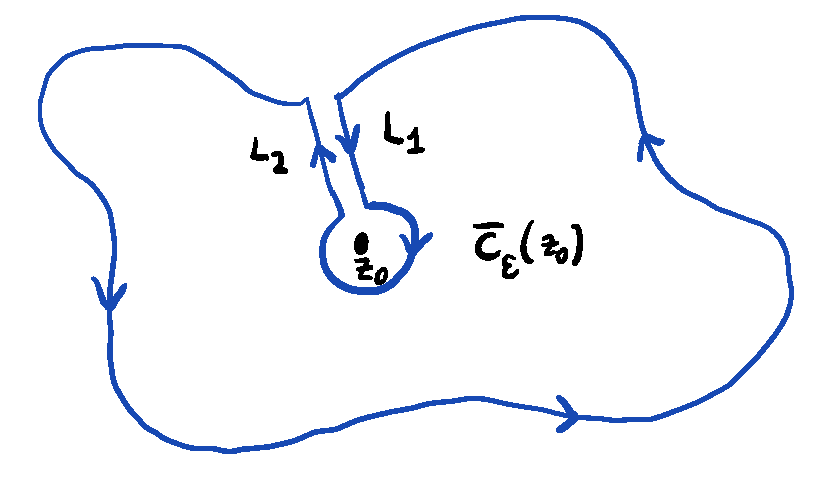
\includegraphics[width=\linewidth]{figs/cauchy_integral-cropped.pdf}
\caption{Contour $C'$ that excises the pole $z_0$ of the
function~\eqref{eq:simplePole}. Following the notation of
\propref{prp:circleIntegral}, $\overline{C}_{\epsilon}(z_0)$ is a circle of
radius $\epsilon$ centered on $z_0$, with the bar indicating that it has a CW
orientation.}
\label{fig:cauchy}
\end{figure}

We choose our excision to have arbitrarily small radius $\epsilon$.
In the limit $\epsilon\to0$, we have
\begin{equation}
  C'=\partial B + L_1 + \overline{C}_{\epsilon}(z_0) + L_2.
\end{equation}
In this limit, $L_1$ and $L_2$ will cancel since they have opposite
orientations.
We can now parameterize $z$ on $\overline{C}_{\epsilon}(z_0)$ 
by $z-z_0=\epsilon e^{i\phi}$, and putting everything together, we find
\begin{equation}\begin{aligned}\label{eq:cauchyn0}
  \oint_{\partial B}\dd{z}\frac{f(z)}{z-z_0}
&=-\lim_{\epsilon\to 0}\int_{2\pi}^0\dd{\phi}
     i\epsilon e^{i\phi}\frac{f(z_0+\epsilon e^{i\phi})}{\epsilon e^{i\phi}}\\
&=i\lim_{\epsilon\to 0}\int_{0}^{2\pi}\dd{\phi}f(z_0+\epsilon e^{i\phi})\\
&=i\int_{0}^{2\pi}\dd{\phi}f(z_0)\\
&=2\pi if(z_0).
\end{aligned}\end{equation}

\index{Cauchy!integral formula}
\begin{theorem}{Cauchy integral formula}{}
Let $B\subset\C$ be bounded and simply connected region. Let $f:B\to\C$ be
holomorphic in $B$ and continuous on the boundary $\partial B$.
Then $\Forall n\in\N$ we get
$$
  \oint_{\partial B}\dd{z}\frac{f(z)}{(z-z_0)^{n+1}}=
\begin{cases}
\frac{2\pi i}{n!}f^{(n)}(z_0) & z_0\in B \\
 0            & \text{otherwise}.
\end{cases}
$$
\begin{proof} When $z_0\notin B$, we get 0 by the Cauchy integral theorem.
Therefore we consider for the remainder of the proof $z_0\in B$.
The $n=0$ case is given by \equatref{eq:cauchyn0}. 
From here, all one has to do is take partial derivatives of this result 
w.r.t. $z_0$.
\end{proof} 
\end{theorem}

\section{The residue theorem}\index{residue!theorem}\label{sec:residueThm}

Let $f$ be holomorphic in the annulus ${z\in\C : 0\leq r<|z-z_0|<R}$
where $r,R>0$.
Define $\Forall\rho : r<\rho<R$ and $\Forall k\in\Z$
\begin{equation}\label{eq:laurentCoeff}
  a_k\equiv\frac{1}{2\pi i}\oint_{C_{\rho}(z_0)}\dd{z}\frac{f(z)}{(z-z_0)^{k+1}}.
\end{equation}
Then the {\it Laurent expansion}\index{Laurent expansion} of $f$ is
\begin{equation}\label{eq:laurentExpansion}
  f(z)=\sum_{k=-\infty}^\infty a_k(z-z_0)^k.
\end{equation}
The $a_k$ are unique and independent of $\rho$, and the Laurent expansion
defines $f$ in the annulus.
If $f$ permits a Taylor expansion, this Taylor series is the Laurent
series, with $a_k=0$ whenever $k<0$.

To get some intuition for why this is true, we can at least show that the
definition~\eqref{eq:laurentCoeff} is consistent.
Plugging \equatref{eq:laurentExpansion} into \equatref{eq:laurentCoeff}
and applying the Cauchy integral formula, we find
\begin{equation}
  a_k\equiv\frac{1}{2\pi i}\sum_{l=-\infty}^\infty\oint_{C_{\rho}(z_0)}
  \dd{z}\frac{a_l}{(z-z_0)^{k-l+1}}
     = \sum_{l=-\infty}^\infty a_l\delta_{k-l,0}=a_k.
\end{equation}

Laurent series can also be used to classify the isolated singularities
of \secref{sec:complexPrelim}. In particular $f$ has at $z_0$
\begin{itemize}
  \item a removable singularity if $a_k=0$ $\Forall k<0$;
  \item a pole of order $m$ if the first, non-vanishing coefficient
        is $a_{-m}$; and
  \item an essential singularity if there is no first, non-vanishing
        coefficient $a_{-m}$.
\end{itemize}

Suppose $f$ has a Laurent expansion in an annulus about $z_0$.
Then the\index{residue} {\it residue} of $f$ at $z_0$ is
\begin{equation}
 \Res f(z_0)=a_{-1}=\frac{1}{2\pi i}\oint_{C_{\rho}(z_0)}\dd{z}f(z).
\end{equation}

\begin{figure}
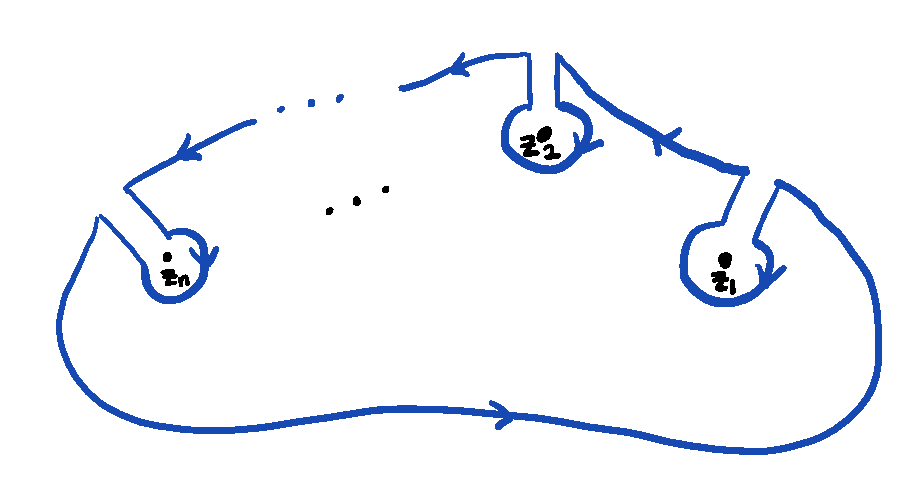
\includegraphics[width=\linewidth]{figs/residue_theorem-cropped.pdf}
\caption{Contour $C'$ that excises all isolated singularities of
the residue theorem. Each singularity is excised by the circle
$\overline{C}_{\rho_k}(z_k)$.}
\label{fig:residue}
\end{figure}

\begin{theorem}{Residue theorem}{residueThm}
Let $B\subset\C$ be an area bounded by a finite number of piecewise
continuous curves. Let $f$ be holomorphic on $\partial B$ 
holomorphic in $B$, except for a finite number of isolated 
singularities $z_1$, ..., $z_n\in B$. Then
$$
\oint_{\partial B}\dd{z}f(z)=2\pi i\sum_{k=1}^n\Res f(z_k).
$$
\begin{proof}
We construct the contour $C'$ indicated in \figref{fig:residue}
created by excising the singularities. Each singularity is
excised with contour $\overline{C}_{\rho_k}(z_k)$, with the
radius $\rho_k$ chosen such that the Laurent expansion
of $f$ converges there. To complete the proof, we use the Laurent
expansion of $f$ around each singularity.
\begin{equation*}
  \oint\dd{z}f(z)=\sum_{k=1}^n\sum_{l=-\infty}^\infty 
                    a_l^{(k)}\oint_{C_{\rho_k}(z_k)}(z-z_k)^l.
\end{equation*}
According to \propref{prp:circleIntegral}, each integral will contribute 
only if $l=-1$; there it contributes $2\pi i$. That the residue is
$a_{-1}$ by definition completes the proof.
\end{proof}
\end{theorem}

\begin{figure}
\centering
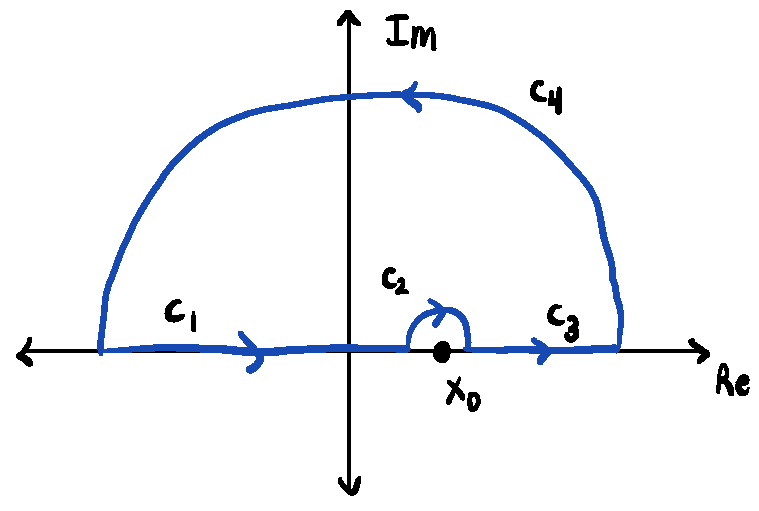
\includegraphics[width=0.75\linewidth]{figs/principal_value-cropped.pdf}
\caption{Example contour used to assign a principal value to a real integral.
Here the semicircle $c_2$ has radius $\epsilon$ and excises the singularity
$x_0$ on the real axis. The semicircle $c_4$ has radius $R$, and the function 
$f$ is asked to decay sufficiently quickly so that the contribution on 
$c_4$ will vanish as $R\to\infty$.}
\label{fig:principalValue}
\end{figure}

The residue theorem is extremely powerful for the evaluation of many integrals,
including real-valued ones. In particular it can be used to assign a number to
a sum of separately divergent, real-valued integrals. 
We begin with an example 
that does not require the residue theorem:
\begin{equation}\label{eq:principalEasy}
  \principal\int_{-a}^a\dd{x}\frac{1}{x}=0
\end{equation} 
with $a>0$, which you can convince yourself of since the integrand is odd. On
the other hand, if one were to split this into a contribution over negative and
positive numbers, each contribution would diverge.

In the above we have introduced the {\it principal value}\index{principal value}
symbol $\principal$. More formally let $f$ be defined in the interval $[a,b]$
with the possible exception $c$, $a<c<b$. Then 
\begin{equation}
  \principal\int_a^b\dd{x}f(x)\equiv\lim_{\epsilon\to0}
     \left(\int_a^{c-\epsilon}\dd{x}f(x)+\int_{c+\epsilon}^b\dd{x}f(x)\right).
\end{equation}

The example~\eqref{eq:principalEasy} was pretty straightforward. A more
interesting example would be
\begin{equation}
  \frac{f(x)}{x-x_0},
\end{equation}
where $f(z)$, $z=x+iy$, has no poles on the real axis. We will also require $f$
to decay in absolute value sufficiently quickly as we move away from the origin.
To determine the principal value, we can use a contour like the one
shown\footnote{If you like, you can also choose $c_2$ to close below the real
axis. Then the singularity $x_0$ will have to be considered in your residue
theorem. The result is the same in either case.}
in \figref{fig:principalValue}. The contours $c_1$ and $c_3$ combine to give
the principal value, and we therefore have by the residue theorem
\begin{equation}
  \principal\int_{-\infty}^{\infty}\dd{x}\frac{f(x)}{x-x_0}
   +\left(\int_{c_2}+\int_{c_4}\right)\dd{z}\frac{f(z)}{z-x_0}
   =2\pi i\sum_k\Res \frac{f(z_k)}{z_k-x_0}. 
\end{equation}
If $f$ decays fast enough, it will vanish on $c_4$, so that term can be
neglected. It remains to evaluate $f$ on $c_2$. We find
\begin{equation}
 \int_{c_2}\dd{z}\frac{f(z)}{z-x_0}
  =\lim_{\epsilon\to0}i\epsilon\int_\pi^0\dd{\phi}
      \frac{f(x_0+\epsilon e^{i\phi})}{\epsilon e^{i\phi}}=-\pi i f(x_0),
\end{equation}
and consequently,
\begin{equation}
  \principal\int_{-\infty}^{\infty}\dd{x}\frac{f(x)}{x-x_0}
   =\pi i f(x_0)+2\pi i\sum_k\Res \frac{f(z_k)}{z_k-x_0}. 
\end{equation}

In the special case where $f$ is analytic in the upper half plane,
there are no residues, and hence
\begin{equation}
  f(x_0)=\frac{1}{\pi i}\,\principal
     \int_{-\infty}^{\infty}\dd{x}\frac{f(x)}{x-x_0}.
\end{equation}
If we write $f(x)=\Re f(x)+i\Im f(x)$, we get from the above
\begin{equation}\begin{aligned}\label{eq:kramerKronig}
\Re f(x_0)&=\frac{1}{\pi}\,\principal
     \int_{-\infty}^{\infty}\dd{x}\frac{\Im f(x)}{x-x_0}\\
\Im f(x_0)&=-\frac{1}{\pi}\,\principal
     \int_{-\infty}^{\infty}\dd{x}\frac{\Re f(x)}{x-x_0}.
\end{aligned}\end{equation}
We call \equatref{eq:kramerKronig} the 
{\it Kramers-Kronig relations}.\index{Kramers-Kronig relations}
They show that the real and imaginary parts of a function $f$ with the given
properties are closely related to each other along the real line.


\section{The Riemann sphere}\index{Riemann sphere}


In this section we introduce a projection of the complex plane called the {\it
Riemann sphere}. It is shown in \figref{fig:riemann}.
The complex plane bisects the Riemann sphere, which is a sphere of unit radius,
and we define a bijective mapping from every point of the $\C$ to the sphere as
follows: Let $(\xi,\eta,\zeta)$ be the coordinates on the surface of the sphere
with respect to its center, so that $\xi^2+\eta^2+\zeta^2=1$.
Then by geometry,
\begin{equation}\label{eq:planeToSphere}
  z=\frac{\xi+i\eta}{1-\zeta},~~~~~~
  \xi+i\eta=\frac{2z}{1+|z|^2},~~~~~~~
  \zeta=\frac{|z|^2-1}{|z|^2+1}.
\end{equation}
The opposite end of a diameter through $(\xi,\eta,\zeta)$ is
$(-\xi,-\eta,-\zeta)$, which corresponds $-1/z^*$.

It is useful to introduce an idea of distance on the Riemann sphere.
A natural choice is the chord length between two points $z$ and $w$
projected onto the sphere. From \equatref{eq:planeToSphere} 
the chord length on the sphere is
\begin{equation}
  D^2(z,w)=\frac{4|z-w|^2}{|1+z^*w|^2+|z-w|^2}.
\end{equation}
This distance satisfies $0<D\leq2$, 
which means we can also about distances to infinity.

This definition of distance can be used to characterize convergence of a
sequence of complex numbers on the sphere. In particular 
a sequence of complex numbers $z_n$ is said to\index{converge!on the sphere}
{\it converge on the sphere} if $\Forall\epsilon>0$ $\Exists N\in\N$
such that
\begin{equation}
  D^2(z_n,z_m)\leq\epsilon^2
\end{equation}
$\Forall n,m\geq N$.

\begin{figure}
\centering
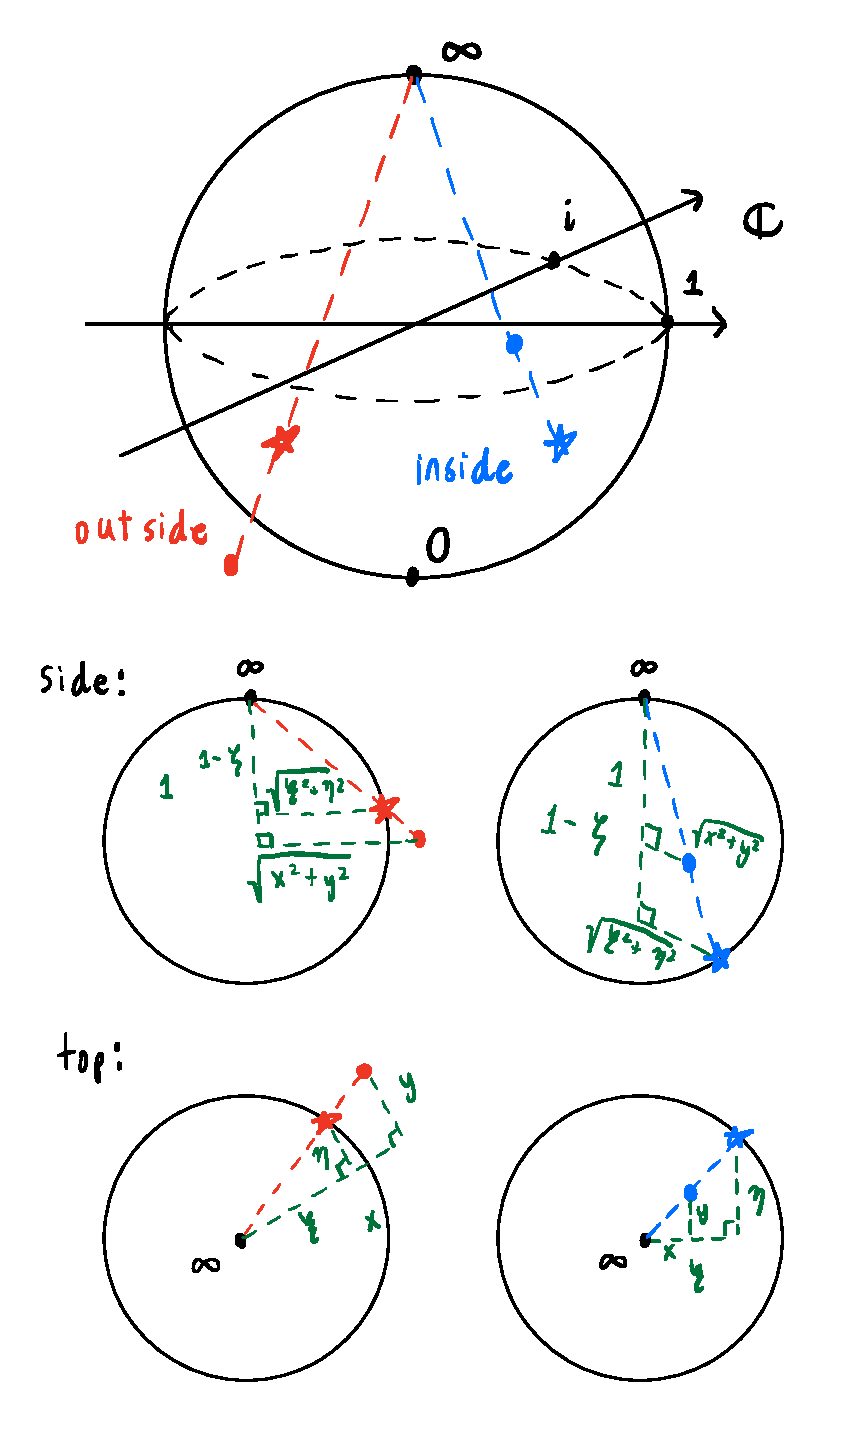
\includegraphics[width=0.7\linewidth]{figs/riemann.pdf}
\caption{{\it Top}: Example mappings of the complex plane to the Riemann sphere.
Filled dots indicate points on the complex planes and stars indicate points on
the surface of the sphere. Hence red lines pierce the sphere and land outside,
while blue lines terminate on the surface. {\it Middle}: A side view of the
Riemann sphere, along with similar triangles to map coordinates on the complex
plane to coordinates on the sphere. {\it Bottom}: Top view of the Riemann
sphere.}
\label{fig:riemann}
\end{figure}


\section{Pad\'e approximants}\index{Pad\'e approximant}

To define the Pad\'e approximant, we introduce\footnote{One can always force
the first coefficient in the denominator to be 1 by factoring it out of all
the other coefficients in both the numerator and denominator.} first the {\it rational
function of order} $[m,n]$, $m,n\in\N$ as \index{function!rational}
\begin{equation}
  R_n^m(x)\equiv\frac{\sum_{i=0}^m a_ix^i}{1+\sum_{j=1}^nb_jx^j}.
\end{equation}
Rational functions can be used instead of Taylor series to approximate
functions with low numbers of terms. They sometimes may have a larger range of
validity than a truncated Taylor series: The intuition is that the coefficients
in the denominator capture some of the contributions from higher order terms.

Let $f$ have a formal Taylor series
\begin{equation}
  f(x)=\sum_{i=0}^\infty c_kx^k.
\end{equation}
Then the {\it Pad\'e approximant} of order $[m,n]$ is the rational function
$R_n^m$ with coefficients so that
\begin{enumerate}
  \item there are no common factors between the numerator and denominator
  \item and it equals the Taylor series up to order $m+n$.
\end{enumerate}
This definition gives a relationship between the coefficients $a_i$, $b_j$, and
$c_k$. We will use this to characterize in which sense Pad\'e approximants
converge to the function they approximate.

Sometimes one does not have access to higher order Taylor coefficients.
One can introduce further constraints by asking that a Pad\'e approximant to agree
with the Taylor series at multiple points, which can be useful if it's easier to
determine lower orders at multiple points than a higher order at a single
one\footnote{This is the situation for lattice determinations of the QCD
pressure expansion in $\mu_B/T$.}. This is the so-called
{\it multi-point Pad\'e}\index{Pad\'e approximant!multi-point}.

\subsection{Rigorous properties}

Here we collect a few known, easy to understand 
facts about Pad\'e approximants. For proofs, we refer
the reader to Ref.~\cite{baker_essentials_1975}. This thorough reference also
contains other useful rigorous properties of Pad\'es. A more up-to-date, brief
article about Pad\'es by the same author can be found in
Ref.~\cite{Jr:2012}.

\begin{theorem}{Uniqueness}{padeUniq}
When it exists, the $[m,n]$ Pad\'e approximant to any Taylor series is unique.
\end{theorem}

\begin{theorem}{Existence}{padeExist}
Given any formal power series with $c_0\neq0$,
then: $\Forall n\in\N$ there exists an infinite sequence of $m_j$ for which the
$[m_j,n]$ Pad\'e exists; $\Forall m\in\N$ there exists an infinite sequence of $n_j$ for
which the $[m,n_j]$ Pad\'e exists; and $\Forall q\in\N$ there exists an infinite
sequence of $m_j$ for which the $[m_j + q/m_j]$ Pad\'e exists.
\end{theorem}

\begin{theorem}{Montessus de Ballore's Theorem}{}
Let $f(z)$ be regular inside the circle $|z|<R$ except for poles of total
multiplicity $n$. Then $\Forall R>0$
the $[m,n]$ Pad\'e converges uniformly
to $f(z)$ on the sphere in $|z|\leq R$ as $m\to\infty$.
\end{theorem}

Montessus de Ballore's theorem guarantees convergence of Pad\'es for meromorphic
functions. It is desirable to use Pad\'es in contexts where functions have more
exotic singularities, for example functions with essential singularities and
branch cuts. Unfortunately it is hard to find practical, rigorous results for
these. For these issues we use numerical experiments to try to glean a few
intuitive or apparent, empirical properties. 


\subsection{Unrigorous properties}



Pad\'e approximants are continuous, except at their poles. That it makes sense
to represent functions with simple poles using Pad\'e approximants is guaranteed
by Montessus de Ballore's theorem. On the other hand,
there may be cases where one constructs a Pad\'e approximant for a function with
an essential singularity or a branch cut, and one may wonder how such
singularities manifest in the approximant.

Since Pad\'e approximants are continuous except at their poles, it must be that
all singularities are somehow represented by poles in the approximant. An
essential singularity, which is an isolated singularity, is represented by a
pole in the approximant. The more interesting case is the branch cut. The only
way the Pad\'e can feel the cut is by a line of poles; in practice it
manifests as a line of alternating zeros and poles. Very intuitively, since
the function value jumps discontinuously from one edge of a Riemann sheet down
to the other edge, maybe one can believe that the best way a rational function
can approximate that is by alternating zeros and poles along the cut. 
The number of points along the cut is limited by the order $n$ of the $[m,n]$ 
approximant, and the rough intuition is that cut is ``recovered" as $n\to\infty$.



\bibliographystyle{unsrtnat}
\bibliography{bibliography}
